\subsection*{Assignment 2.g \hrule}
\textbf{Question}
\begin{quote}
Take the radial bin from assignment 2.e containing the largest number of galaxies. Using sorting, calculate the median, 16th and 84th percentile for this bin and output these values. Next, make a histogram of the number of galaxies in this radial bin in each halo (so 1000 values), each bin of this histogram should have a width of 1. Plot this histogram, and over-plot the Poisson distribution with $\lambda$ equal to the mean number of galaxies in this radial bin.
\end{quote}

\textbf{Solution}
\begin{quote}

The code does for this exercise  consists of three files. The first file (\textsf{./code/assignment2\_ g.py}) contains the code that creates the plot and prints the output. The second file (\textsf{./code/mathlib/sorting.py}) contains the code for merge sorting. The last file (\textsf{./code/mathlib/utils.py}) contains the functions for the median, percentile and Poisson distribution. A part of this last file has earlier been shown in assignment 1.b. The full file, inclusive the earlier shown part, can be found below. 

% and the percentile. This last file also contains other functions that have previously bee 
%n the array of the 84 th percentile is not an integer (i.e index = 5.54), then lineair interpolate the value at index 5 and at index 6 to estimate the value at index 5.54. 
\end{quote}
\newpage

\textbf{Code - output}
\begin{quote}
The code that produces the output.
\lstinputlisting{./code/assignment2_g.py}
\end{quote}

\textbf{Code - merge sort}
\begin{quote}
The code for merge sort that is used for the median and the percentile.
\lstinputlisting[lastline=71]{./code/mathlib/sorting.py}
\end{quote}

\textbf{Code - Poisson, median, percentile}
The code of the Poisson distribution, median function and percentile function.
\begin{quote}
\lstinputlisting{./code/mathlib/utils.py}
\end{quote}

\textbf{Output - text}
\begin{quote}
The text output from \textsf{./code/assignment2\_ g.py}
\lstinputlisting{./output/assignment2_g_out.txt}
\end{quote}

\newpage

\textbf{Output - figure}
\begin{quote}
The plot created in \textsf{./code/assignment2\_ g.py}
\begin{figure}[!h]
\centering
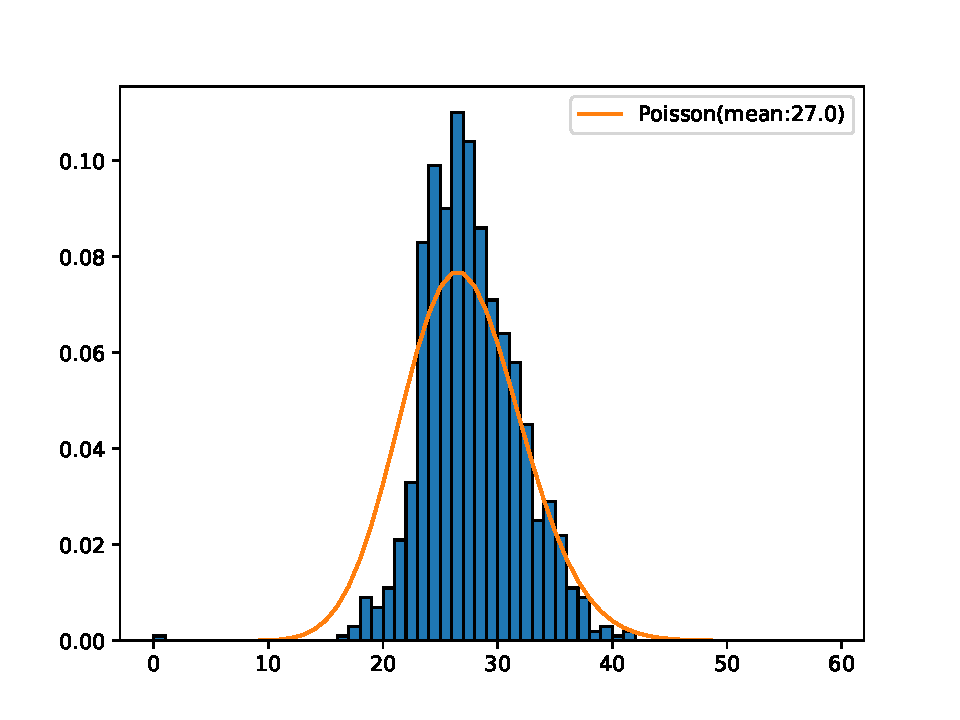
\includegraphics[scale=0.7]{plots/poisson.pdf}
\caption{The Poisson distribution over-plotting the created histogram. The figure shows that the number of satellites on a spherical shell at a distance x is approximately distributed according to a Poisson distribution around N(x) - the number of satellites predicted by the model on an infinite thin spherical shell. }
\end{figure}
\end{quote}












